
\documentclass{article}
\usepackage{tikz}
\usetikzlibrary{shapes.geometric, arrows, positioning}

\begin{document}
\thispagestyle{empty}
\begin{center}
\resizebox{\textwidth}{!}{
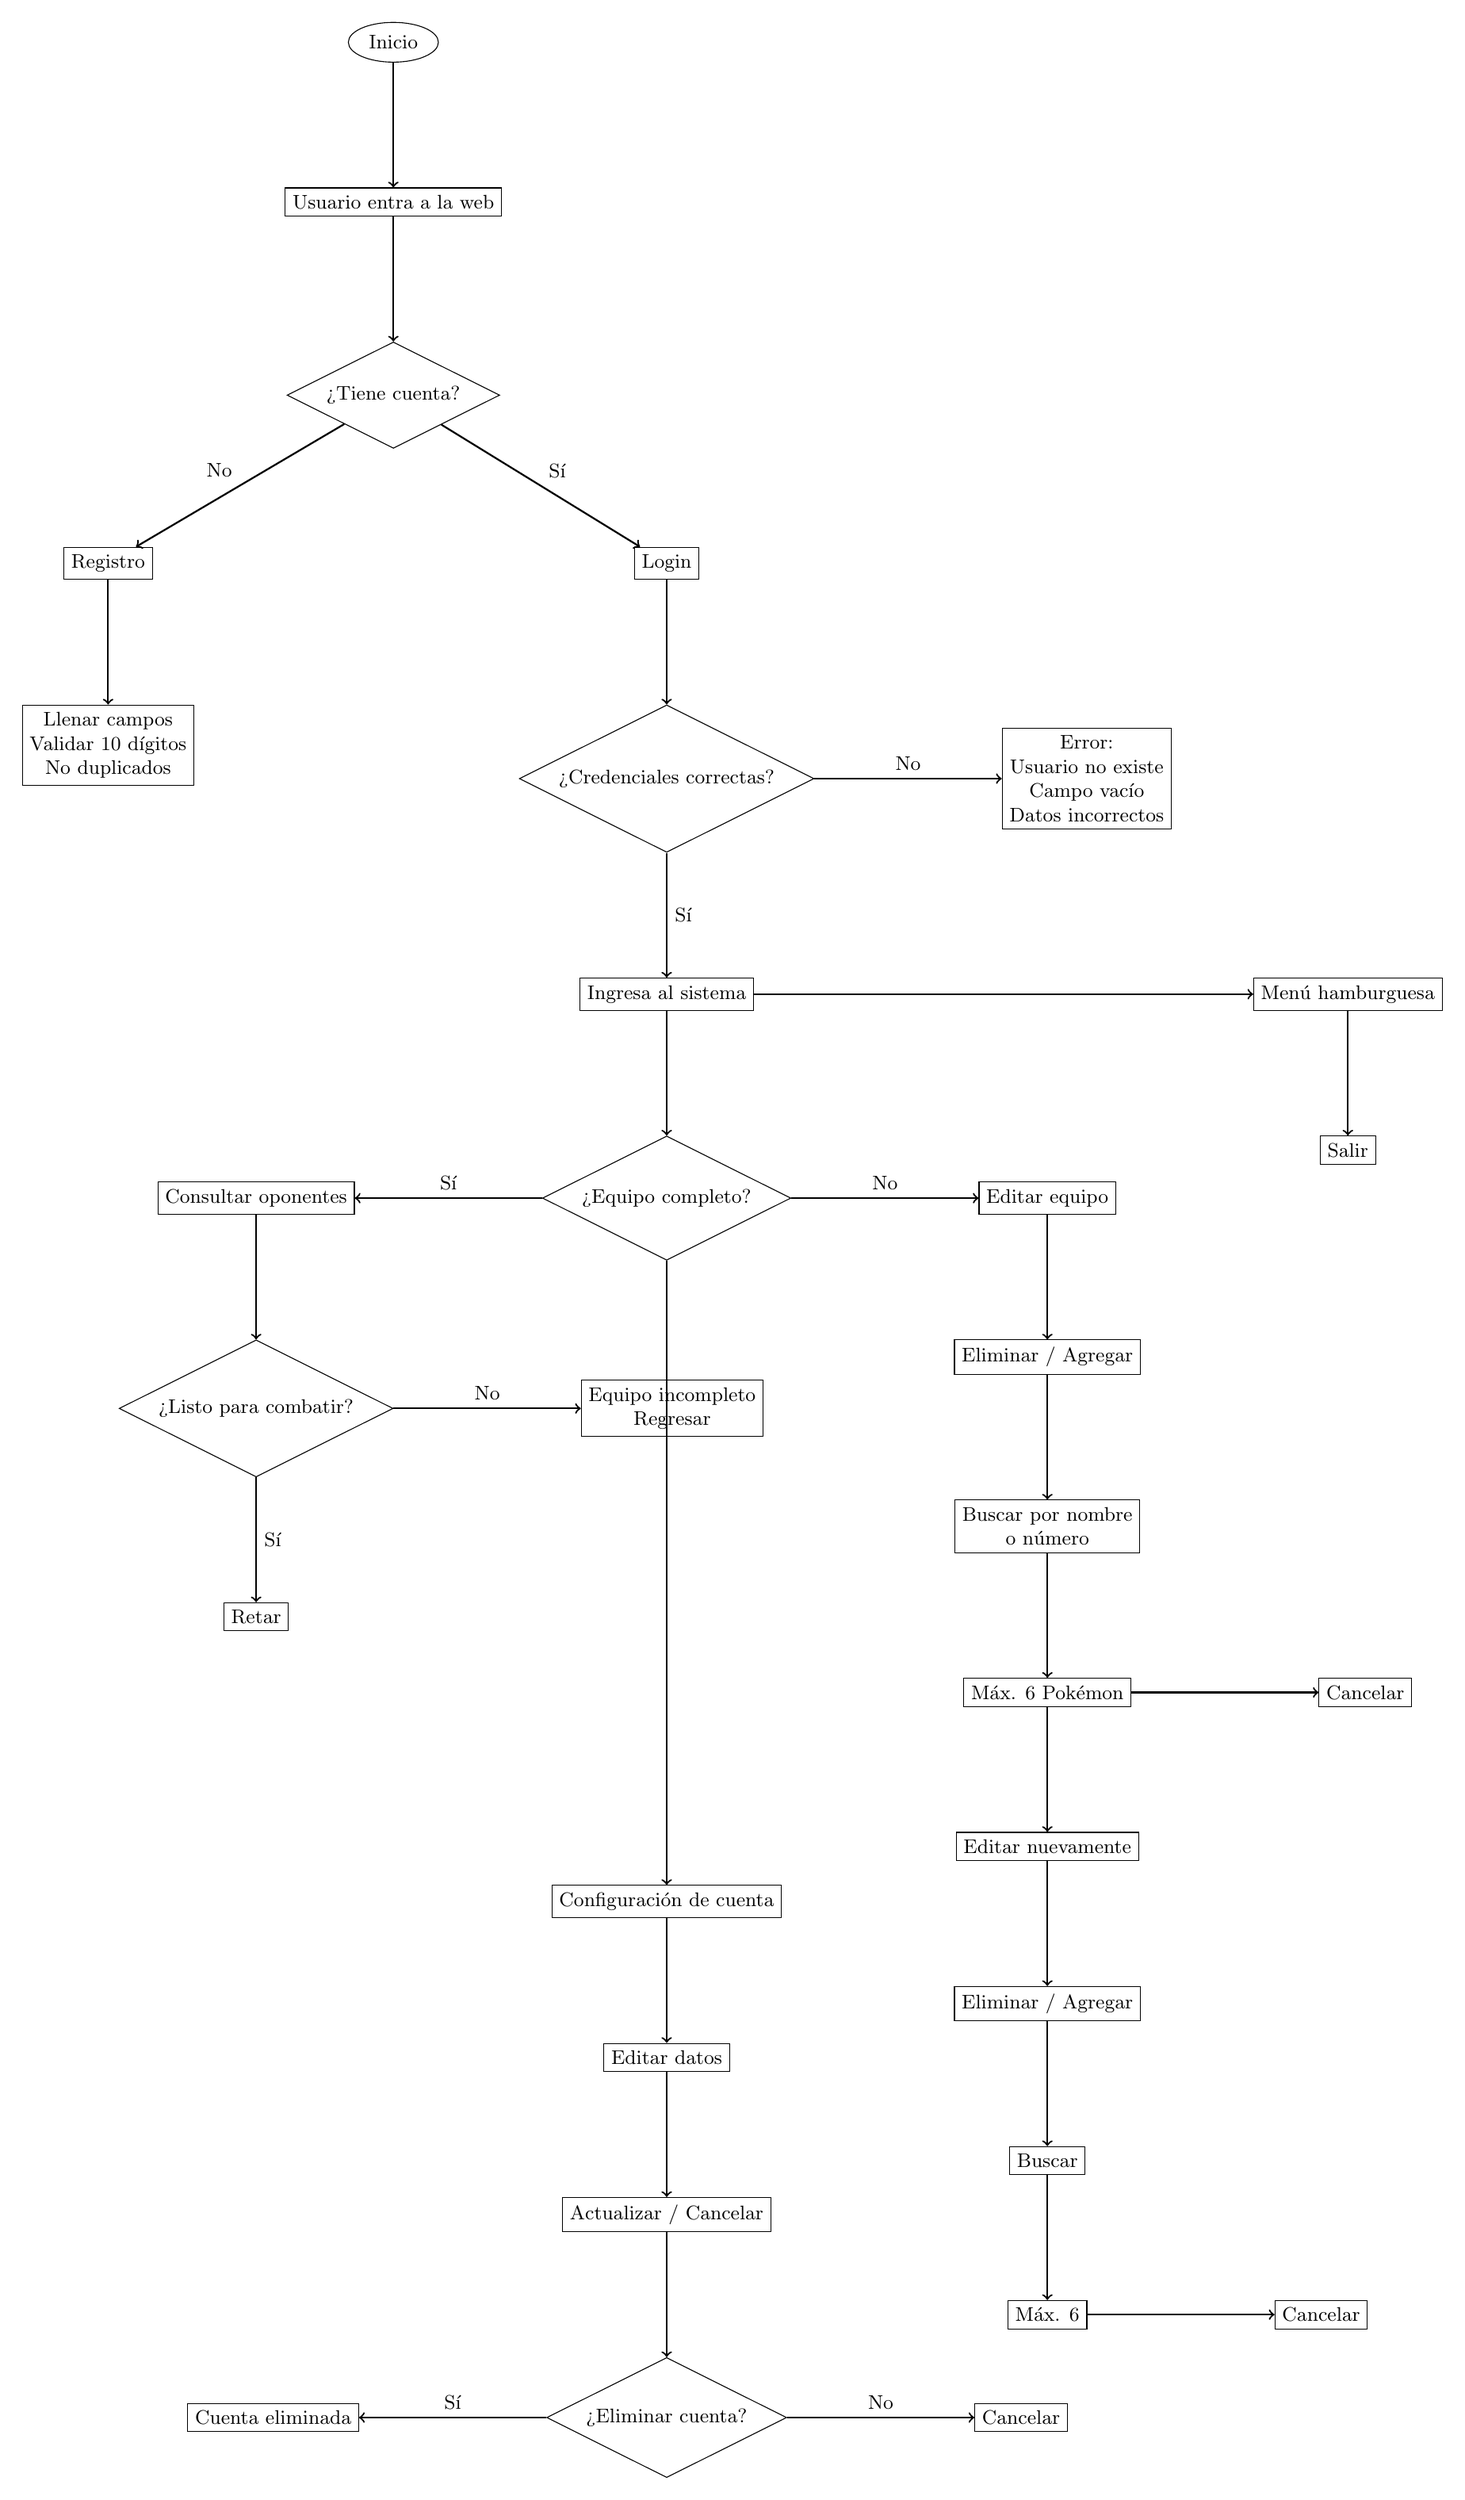
\begin{tikzpicture}[
node distance=2cm and 3cm,
every node/.style={align=center, font=\small},
startstop/.style={ellipse, draw},
process/.style={rectangle, draw},
decision/.style={diamond, draw, aspect=2},
arrow/.style={->, thick}
]

% INICIO
\node (inicio) [startstop] {Inicio};
\node (web) [process, below=of inicio] {Usuario entra a la web};
\node (cuenta) [decision, below=of web] {¿Tiene cuenta?};

% REGISTRO
\node (registro) [process, below left=of cuenta] {Registro};
\node (validacion) [process, below=of registro] {Llenar campos\\Validar 10 dígitos\\No duplicados};

% LOGIN
\node (login) [process, below right=of cuenta] {Login};
\node (credenciales) [decision, below=of login] {¿Credenciales correctas?};
\node (error) [process, right=of credenciales] {Error:\\Usuario no existe\\Campo vacío\\Datos incorrectos};
\node (sistema) [process, below=of credenciales] {Ingresa al sistema};

% EQUIPO
\node (equipo) [decision, below=of sistema] {¿Equipo completo?};

% SI equipo completo
\node (oponentes) [process, left=of equipo] {Consultar oponentes};
\node (listo) [decision, below=of oponentes] {¿Listo para combatir?};
\node (retar) [process, below=of listo] {Retar};
\node (noListo) [process, right=of listo] {Equipo incompleto\\Regresar};

% NO equipo completo (editar equipo)
\node (editar1) [process, right=of equipo] {Editar equipo};
\node (acciones1) [process, below=of editar1] {Eliminar / Agregar};
\node (buscar1) [process, below=of acciones1] {Buscar por nombre\\o número};
\node (max1) [process, below=of buscar1] {Máx. 6 Pokémon};
\node (cancelar1) [process, right=of max1] {Cancelar};

% EDICION ADICIONAL (cuando ya tiene pero quiere editar)
\node (editar2) [process, below=of max1] {Editar nuevamente};
\node (acciones2) [process, below=of editar2] {Eliminar / Agregar};
\node (buscar2) [process, below=of acciones2] {Buscar};
\node (max2) [process, below=of buscar2] {Máx. 6};
\node (cancelar2) [process, right=of max2] {Cancelar};

% CONFIGURACION
\node (config) [process, below=of equipo, yshift=-8cm] {Configuración de cuenta};
\node (editarDatos) [process, below=of config] {Editar datos};
\node (actualizar) [process, below=of editarDatos] {Actualizar / Cancelar};
\node (eliminarCuenta) [decision, below=of actualizar] {¿Eliminar cuenta?};
\node (borrar) [process, left=of eliminarCuenta] {Cuenta eliminada};
\node (cancelarCuenta) [process, right=of eliminarCuenta] {Cancelar};

% MENU
\node (menu) [process, right=of sistema, xshift=5cm] {Menú hamburguesa};
\node (salir) [process, below=of menu] {Salir};

% FLECHAS
\draw[arrow] (inicio) -- (web);
\draw[arrow] (web) -- (cuenta);

% Registro
\draw[arrow] (cuenta) -- node[above left]{No} (registro);
\draw[arrow] (registro) -- (validacion);

% Login
\draw[arrow] (cuenta) -- node[above right]{Sí} (login);
\draw[arrow] (login) -- (credenciales);

\draw[arrow] (credenciales) -- node[right]{Sí} (sistema);
\draw[arrow] (credenciales) -- node[above]{No} (error);

% Sistema → equipo
\draw[arrow] (sistema) -- (equipo);

% Equipo SI
\draw[arrow] (equipo) -- node[above]{Sí} (oponentes);
\draw[arrow] (oponentes) -- (listo);
\draw[arrow] (listo) -- node[right]{Sí} (retar);
\draw[arrow] (listo) -- node[above]{No} (noListo);

% Equipo NO
\draw[arrow] (equipo) -- node[above]{No} (editar1);
\draw[arrow] (editar1) -- (acciones1);
\draw[arrow] (acciones1) -- (buscar1);
\draw[arrow] (buscar1) -- (max1);
\draw[arrow] (max1) -- (cancelar1);

% Edición adicional
\draw[arrow] (max1) -- (editar2);
\draw[arrow] (editar2) -- (acciones2);
\draw[arrow] (acciones2) -- (buscar2);
\draw[arrow] (buscar2) -- (max2);
\draw[arrow] (max2) -- (cancelar2);

% Configuración
\draw[arrow] (equipo) -- (config);
\draw[arrow] (config) -- (editarDatos);
\draw[arrow] (editarDatos) -- (actualizar);
\draw[arrow] (actualizar) -- (eliminarCuenta);
\draw[arrow] (eliminarCuenta) -- node[above]{Sí} (borrar);
\draw[arrow] (eliminarCuenta) -- node[above]{No} (cancelarCuenta);

% Menu paralelo
\draw[arrow] (sistema) -- (menu);
\draw[arrow] (menu) -- (salir);

\end{tikzpicture}
}
\end{center}

\end{document}

